\documentclass[a4paper,12pt]{report}
\usepackage[utf8]{inputenc}
\usepackage[frenchb]{babel}
\usepackage[T1]{fontenc}
\usepackage{lmodern,textcomp}
\usepackage{graphicx}
\usepackage{listings}
\usepackage{caption}
\usepackage{fancybox}
\usepackage[pdftex]{hyperref}
\usepackage[usenames,dvipsnames]{pstricks}
\usepackage{epsfig}
\usepackage{fancyvrb}
\usepackage{alltt}

\hypersetup{%
  colorlinks= true,
  linkcolor = blue
  }
\hypersetup{
  pdftitle={Xia},
  pdfauthor={Énuma Logiciel Libre},
  pdfsubject={Xia},
  pdfkeywords={Xia, logiciel libre, html5, Inkscape}
}

\renewcommand{\thechapter}{\arabic{chapter}}
\renewcommand{\thesection}{\Roman{section}}
\renewcommand{\thesubsection}{\alph{subsection}}

% pour unifier les indications relatives aux manipulation à effectuer dans les logiciels
% à modifier au besoin
\newcommand{\chemin}[1]{\textcolor{red}{#1}}

\begin{document}
 
 \tableofcontents
 
 % il y a, à plusieurs reprises, des paragraphes du style "<à noter"> ou "<astuces">
 % peut-être faut-il adopter le style utilisé pour ce genre de choses dans la doc se3?
 
\section{Présentation de Xia}

\subsection{Qu'est-ce que Xia?}

Xia est un logiciel libre développé par la délégation académique pour le numérique éducatif de l'académie de Versailles.
Distribué sous licence \href{http://www.gnu.org/copyleft/gpl.html}{GPLv3}, il est le successeur du logiciel «~ImagesActives~».
Xia est un convertisseur qui prend en entrée un fichier svg et fournit en sortie une image active en html5.
Au-delà des templates d'export déjà connus des utilisateurs du logiciel ImagesActives
(\href{http://images-actives.crdp-versailles.fr/spip.php?article11&lang=fr}{accordéon, boutons, etc.}),
Xia permet en outre de générer des activités interactives: jeux de glisser-déposer, discrimination, sélection, etc.

Cette documentation est un guide «~pas à pas~» pour la réalisation d'images actives.
Partant de la réalisation d'une image active simple (détourage et commentaires sans enrichissements particuliers)
elle guide l'utilisateur vers la réalisation d'images plus complexes (enrichissements multimédias, jeux, etc.)
Les exemples sont visibles en ligne (le lien est signalé en début de section), les fichiers sources (au format svg) 
sont également téléchargeables. À la fin de chaque partie, une rubrique «~Pour résumer~» reprend de manière 
synthétique les grands principes à retenir pour la fabrication d'images actives.

\subsection{Processus général}

Contrairement à ImagesActives, Xia n'intervient qu'en toute fin de processus de création de la ressource.
Comme on peut le constater sur la figure \ref{workflow_xia}, l'essentiel du travail est à effectuer
dans un logiciel de dessin vectoriel.
Nous recommandons fortement l'utilisation d'\href{http://www.inkscape.org/}{Inkscape}, logiciel libre
multi-plateforme, très aisé à prendre en main, et qui sera utilisé dans cette documentation.

\begin{figure}[htp]
 \centering
 \caption{Processus de création d'une image active avec Xia}
 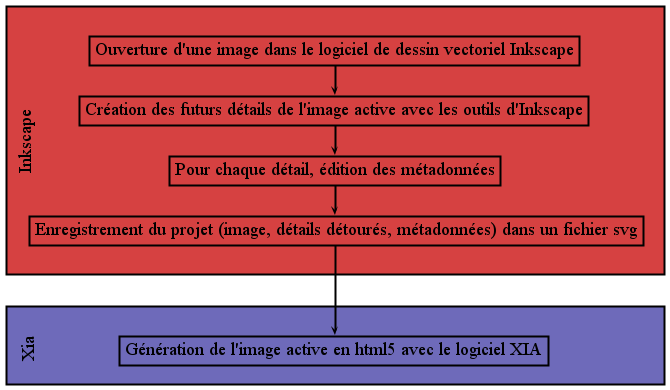
\includegraphics[width=1\textwidth]{images/workflow_xia}
 \label{workflow_xia}
\end{figure}

\section{Réalisation d'une première image active avec Inkscape et Xia: fonctionnalités de base}

\subsection{Installation d'Inkscape et de Xia}

L'installation d'Inkscape et de Xia est le seul pré-requis à la suite de la lecture de cette documentation.
Les informations nécessaires à ces manipulations se trouvent sur les sites respectifs des projets\footnote{Voir les sites d'\href{http://www.inkscape.org/}{Inkscape} et de \href{http://images-actives.crdp-versailles.fr/beta/}{Xia}.}.

\subsection{Préparation du fichier svg en vue de la génération de l'image active}\label{preparation_svg}

% cette phrase est répétée en début de chaque section: il faudrait trouver un moyen de la mettre en valeur
Explorez l'\href{http://geoffrey-gekiere.ac-versailles.fr/xia1}{image active créée pour cette section de la documentation} 
et téléchargez le \href{http://geoffrey-gekiere.ac-versailles.fr/xia1/svg/xia1.svg}{svg}.

Les quelques manipulations décrites dans cette section sont suffisantes
pour réaliser une image active «~de base~»
ayant les caractéristiques suivantes:
\begin{itemize}
 \item Détails zoomables
 \item Commentaires des détails constitués uniquement de texte non mis en forme
\end{itemize}


Une fois l'image à travailler choisie, on l'ouvre dans Inkscape (menu \chemin{Fichier} puis \chemin{Ouvrir}).
À la question posée par le logiciel («~\chemin{Lier ou incorporer l'image}~»), on choisira «~\chemin{Incorporer}~».

Parmi les nombreuses informations que l'on peut renseigner en accédant à la fenêtre de dialogue des 
\chemin{Métadonnées du document} (menu \chemin{Fichier}), trois seront prises en compte dans l'image active
une fois générée: le titre, le créateur, les droits.
Il est donc fortement recommandé de les renseigner.
Dans l'exemple suivant (voir figure \ref{titre_ia}), on voit l'importance d'un titre correctement
renseigné dans les métadonnées: il s'agit en réalité du titre de l'image active\footnote{Les champs 
«~auteur~» et «~droits~» apparaissent pour leur part dans la fenêtre «~À propos~», symbolisé par 
un bouton clicable en forme de lettre «~i~».}.

\begin{figure}[htp]
 \centering
 \caption{Le titre renseigné dans les métadonnées du document apparaît au-dessus de l'image active 
 et donne son nom à la page web de celle-ci, le créateur et les droits associés apparaissent dans la pop up
 associée au bouton «~i~» situé à droite du titre de l'image active}
 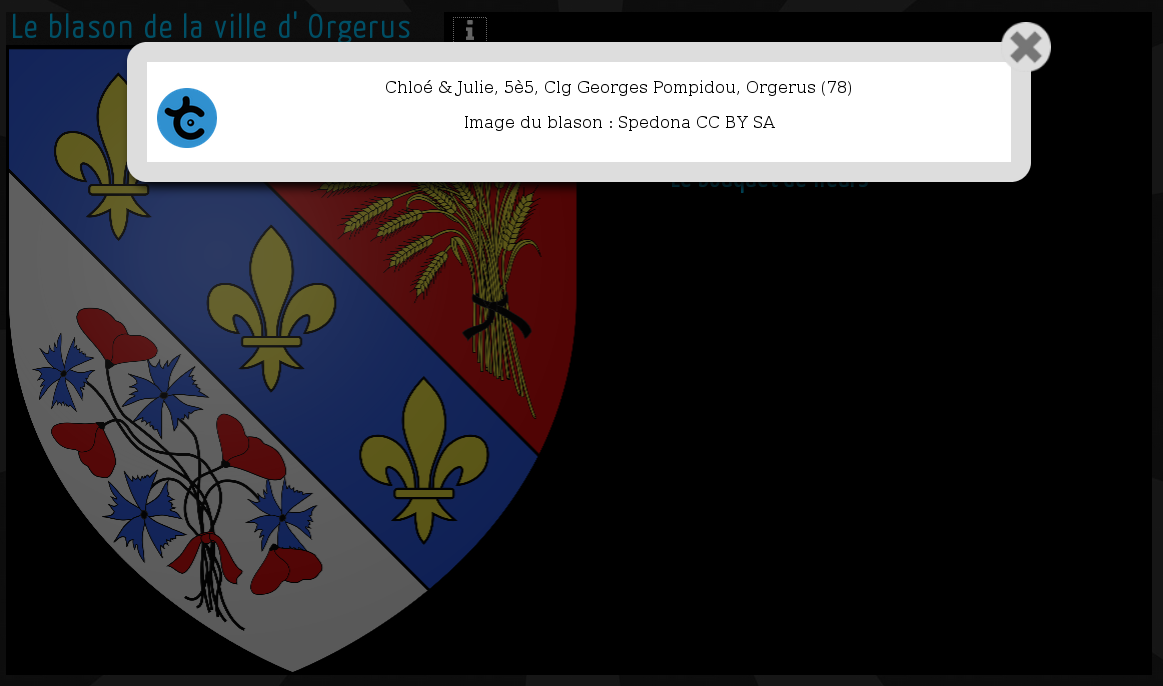
\includegraphics[width=\textwidth]{images/titre_ia}
 \label{titre_ia}
\end{figure}

On peut enregistrer l'image au format svg dès le début du travail, en
passant par le menu \chemin{Fichier} puis \chemin{Enregistrer sous...}.
Pour davantage de lisibilité, on supprimera l'extension actuelle de l'image dans le champs \chemin{Nom} 
 de la fenêtre de dialogue. Enfin, dans le menu déroulant permettant de choisir le format de 
 fichier: format \chemin{SVG Inkscape (*.svg)}.

Plusieurs outils d'Inkscape sont utilisables pour détourer les détails qui deviendront actifs dans l'image générée 
par Xia. Parmi ceux-ci:
\begin{itemize}
 \item 
\includegraphics[scale=0.5]{./images/rec_carre} L'outil \chemin{Créer des rectangles et des carrés}
 \item 
\includegraphics[scale=0.5]{./images/cercles} L'outil \chemin{Créer des cercles, des ellipses et des arcs}
 \item 
\includegraphics[scale=0.5]{./images/lignes} L'outil \chemin{Dessiner des lignes à main levée}
 \item 
\includegraphics[scale=0.5]{./images/bezier} L'outil \chemin{Tracer des courbes de Bézier et des segments de droite}
\end{itemize}

% dans ce paragraphe, peut-être insérer une bidouille quelconque pour que l'allusion aux touches
% Ctrl et Maj soit plus claire (dessiner une touche de clavier?)
Sans rentrer dans le détail du fonctionnement de ces outils\footnote{Pour cela, 
se référer au \href{http://inkscape.org/doc/shapes/tutorial-shapes.fr.html}{manuel d'Inkscape}.}, on notera cependant que
les outils «~\chemin{Créer des rectangles et des carrés}~» et «~\chemin{Créer des cercles, des ellipses et des arcs}~»
 peuvent se manipuler uniquement à la souris ou en lien avec le clavier: en appuyant sur la touche Ctrl, on 
 dessine un carré, rectangle ou cercle de rapport de dimensions entier (2:1, 3:1, etc.),
 et en appuyant sur la touche Maj, on dessine autour du point de départ.

L'outil «~\chemin{Tracer des courbes de Bézier et des segments de droite}~» permet de détourer «~clic par clic~»
(on appelle les points de construction des «~nœuds~»).
On referme la figure en cliquant sur le nœud de départ.
L'outil «~courbe de bézier~» est appelé en gardant le clic de souris appuyé après avoir créé un nœud, 
puis en déplaçant le pointeur pour faire apparaitre les poignées de contrôle permettant de modeler
le segment de courbe à volonté.

À noter:
\begin{itemize}
 \item si l'utilisateur définit dans Inkscape une forme laissée ouverte (par exemple: une ligne),
Xia la «~refermera~» automatiquement en reliant par une droite le début et la fin de celle-ci.
 \item l'ordre de création des détails correspond dans l'image générée à l'ordre d'affichage des détails
 (par exemple, le détail créé en premier dans Inkscape apparaîtra en haut dans l'image active)\footnote{Pour modifier 
 l'ordre sans avoir à recréer les détails, voir la section \ref{couche_XML}.}
\end{itemize}

Une fois un détail détouré, on le sélectionne avec l'outil 
\chemin{Sélectionner et transformer des objets} afin de le redimensionner, le déplacer, etc.

C'est par un clic droit sur le détail détouré que l'on accède aux \chemin{Propriétés de l'objet} (voir figure \ref{proprietes_objet}),
et ainsi à la fenêtre de dialogue dans laquelle on renseigne le texte qui sera associé au détail dans l'image active
une fois générée.

\begin{figure}[htp]
 \centering
 \caption{Accès aux «~Propriétés de l'objet~», permettant de renseigner le texte 
 qui servira de commentaire au détail dans l'image active générée}
 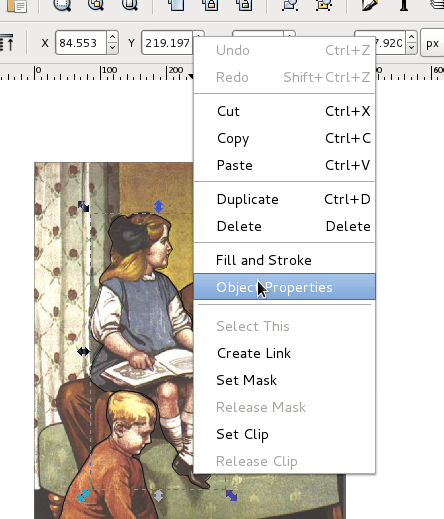
\includegraphics[width=0.5\textwidth]{./images/proprietes_objet}
 \label{proprietes_objet}
\end{figure}

Les deux champs à renseigner dans cette fenêtre sont \chemin{Titre} et \chemin{Description}.
Le titre renseigné ici sera celui du détail, la description en sera son commentaire.

Le processus décrit ci-dessus doit également être réalisé avec l'image de fond: le titre et la description renseignées
serviront d'introduction à l'image active (titre et commentaire non reliée à un détail particulier).

\subsection{Génération de l'image active dans Xia}

\begin{figure}[htp]
 \centering
 \caption{Vue générale de l'interface du logiciel Xia}
 
\includegraphics[width=0.8\textwidth]{./images/xia_vue_generale}
 \label{xia_interface}
\end{figure}

Quand tous les détails sont détourés et leurs métadonnées renseignées, on peut lancer le logiciel Xia (voir la figure \ref{xia_interface}).
La première icône, en haut à gauche, permet de choisir le fichier svg à générer:
\begin{center}

\includegraphics[scale=0.4]{./images/xia_open} 
\end{center}

Un clic sur l'une des icônes d'export génère une série de fichiers, dont un \verb|index.html|. 
Attention: ce fichier seul est inexploitable. Tous les autres fichiers et répertoires générés lors de l'export 
sont indispensables au bon fonctionnement de l'animation. \textbf{Il est donc indispensable de dédier un répertoire 
spécifique à chaque image exportée, afin d'éviter des déconvenues}.
Il suffit cependant d'ouvrir le fichier \verb|index.html| dans un navigateur pour voir apparaître l'image active.

Les templates d'images actives «~simples~» sont les suivants:
% pertinence d'ajouter une 4e colonne pour décrire brièvement les caractéristiques de chaque export?
\begin{center}
\begin{tabular}{|c|c|p{3in}|}
\hline
Thème & Icône & Caractéristiques à retenir\\
\hline
\href{http://geoffrey-gekiere.ac-versailles.fr/xia1/accordionBlack}{accordionBlack}  & 
\includegraphics[scale=0.5]{./images/accordionBlack} & Zone de commentaire large, utile pour l'insertion de ressources multimédias; à privilégier pour les images en format portrait\\
\hline
\href{http://geoffrey-gekiere.ac-versailles.fr/xia1/accordionCloud}{accordionCloud} &  
\includegraphics[scale=0.5]{./images/accordionCloud}& Zone de commentaire étroite, laissant davantage de place à l'image en elle-même; à privilégier pour les images en format paysage\\
\hline
\href{http://geoffrey-gekiere.ac-versailles.fr/xia1/buttonBlue}{buttonBlue}&  
\includegraphics[scale=0.5]{./images/buttonBlue} & Image apparaissant en pleine largeur; les commentaires des détails apparaissent dans une pop up au-dessus de l'image active (utile pour les commentaires longs); les détails sont accessibles par un bandeau numéroté situé au-dessus de l'image active\\
\hline
\href{http://geoffrey-gekiere.ac-versailles.fr/xia1/popBlue}{popBlue} &  
\includegraphics[scale=0.5]{./images/popBlue} & L'image apparaît en pleine largeur; un premier clic fait apparaître le détail, un second le commentaire au-dessus de l'image active (le zoom est désactivé)\\
\hline
\href{http://geoffrey-gekiere.ac-versailles.fr/xia1/popYellow}{popYellow} &  
\includegraphics[scale=0.5]{./images/popYellow} & L'image apparaît en pleine largeur; un premier clic fait apparaître le détail, un second déclenche simultanément l'apparition du commentaire et le zoom sur le détail\\
\hline
\end{tabular}
\end{center}

\subsection{Pour résumer}

\begin{enumerate}
 \item Une image active est conçue dans le logiciel Inkscape, au format .svg, 
 Xia transforme ce svg en animation au format html5
 \item Le titre de l'image active est renseigné dans les \chemin{Métadonnées du document}
 \item Le texte des détails est renseigné dans les \chemin{Propriétés de l'objet},
 champs \chemin{Titre} et \chemin{Description}
 \item La description générale de l'image active est renseignée dans les \chemin{Propriétés de l'objet} 
 de l'image de fond
\end{enumerate}

\section{Image active enrichie}

Explorez l'\href{http://geoffrey-gekiere.ac-versailles.fr/xia2}{image active créée pour cette section de la documentation} 
et téléchargez le \href{http://geoffrey-gekiere.ac-versailles.fr/xia2/svg/xia2.svg}{svg}.

Dans cette section, nous réalisons toujours une image active classique (un détail = un commentaire),
mais nous enrichissons le contenu de celle-ci par divers moyens, comme une mise en forme avancée du texte ou des contenus 
multimédias directement insérés dans les commentaires.

\subsection{Mise en forme du texte}

Pour mettre en forme le texte des commentaires, on insérera les balises suivantes:

% problème d'alignement du contenu des cellules sur les lignes "<liste de puces"> et "<tracer une ligne">
\begin{center}
 \begin{tabular}{|l|l|}
 \hline
  Balises & Résultat\\
  \hline
  \hline
  ***gras*** & \textbf{gras}\\
  \hline
  **italique** & \textit{italique}\\
  \hline
  [http://dane.ac-versailles.fr Le site de la Dane] & \href{http://dane.ac-versailles/fr}{Le site de la Dane}\\
  \hline
  \{\{\{Texte brut\}\}\} & 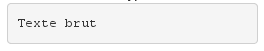
\includegraphics[scale=0.7]{./images/texte_brut}\\
  % là, faudrait symboliser les espaces simple et double pour les listes de puces
  \hline
  ~* une liste\\
  ~* de puces\\
  ~~* sur 2\\
  ~~* niveaux\\ & 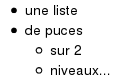
\includegraphics[scale=0.7]{./images/liste_puce}\\
  \hline
  tracer\\
  \verb|----|\\
  une ligne\\ & 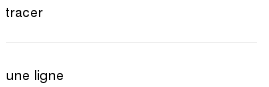
\includegraphics[scale=0.7]{./images/ligne_commentaire}\\
  \hline
  \end{tabular}
\end{center}

\subsection{Enrichissement multimédia des détails}\label{enrichissement_multimedia}

L'insertion de contenus multimédias dans les commentaires des détails est extrêmement aisée:
il suffit à l'utilisateur d'indiquer l'url (relative ou absolue) de la ressource, ou d'insérer le code iframe
fourni par le service hébergeant le contenu (par exemple, la \href{https://scolawebtv.crdp-versailles.fr/}{Scolawebtv}).

Nativement, Xia génère un lecteur multimédia dans le commentaire à partir du moment où la ressource (image, son ou vidéo)
correspond à un des formats suivants:
\begin{description}
 \item [Images] jpg, jpeg, png, gif
 \item [Son] ogg, mp3
 \item [Vidéo] ogv, webm, mp4
\end{description}

Le lien est simplement inséré dans le fil du commentaire du détail:
\begin{description}
 \item [Lien absolu] Si la ressource se trouve à l'adresse\\
 \begin{center}
 \verb|http://web.crdp.ac-versailles.fr/02546.ogg|\\
 \end{center}
 il suffira d'indiquer cette adresse dans le champs description des propriétés de l'objet, dans Inkscape
 \item [Lien relatif] Si la ressource se trouve dans le dossier d'export ou dans un dossier situé dans le dossier d'export, on en indiquera
 l'emplacement en considérant le dossier d'export comme la racine. Par exemple, si \verb|video.ogv| se trouve dans un répertoire \verb|videos| lui-même situé dans le dossier d'export, on indiquera dans
 le commentaire\\
 \begin{center}
  \verb|videos/video.ogv|
 \end{center}
  pour que le lecteur soit créé
\end{description}

Les différents formats vidéos gérés par Xia ne sont pas nativement reconnus par tous les navigateurs.
Une méthode pour contourner ce problème peut consister à exporter dans les trois formats la ressource,
et à déposer les trois fichiers ainsi obtenus dans un répertoire identique, avec le même nom (seule l'extension
en .ogv, .mp4 et .webm les différencie alors):\\

% je pense qu'il y a moyen de faire vachement plus joli pour représenter l'arborescence
 % po4a: environment tikzpicture {} 
\begin{tikzpicture}
\end{tikzpicture}
 % po4a: environment alltt {} 
\parbox{0.40\textwidth}
{
\begin{alltt}
 -\textcolor{blue}{repertoire\_export}\\
 ---index.html\\
 ---[ensemble des fichiers et répertoires générés par Xia]\\
 ---\textcolor{blue}{repertoire\_videos}\\
 -----video.mp4\\
 -----video.ogv\\
 -----video.webm\\
\end{alltt}
}
\fbox{\begin{minipage}{0.50\textwidth}
	Dans l'exemple ci-contre, les répertoires, en bleu, ont été créés par l'utilisateur. 
	Dans le répertoire \textcolor{blue}{repertoire\_export}
	se trouvent les répertoires et fichiers générés par Xia, dont le fichier index.html.
	On crée également dans ce répertoire un répertoire \textcolor{blue}{repertoire\_videos} qui a pour fonction
	de stocker les vidéos qui seront appelées dans les commentaires de l'image active grâce à un lien relatif.
      \end{minipage}}


Ainsi, même si un format particulier est indiqué dans la description (en suivant l'exemple précédent: \verb|repertoire_videos/video.ogv|),
si le navigateur ne parvient pas à lire la ressource, il tentera automatiquement de lire les fichiers du même nom 
possèdant une extension différente (soit, ici, \verb|video.mp4| puis \verb|video.webm|).

Enfin, la dernière possibilité consiste à insérer dans le commentaire le code iframe d'un service d'hébergement de ressources.
Celui-ci sera interprêté et le lecteur du service s'affichera dans le commentaire, donnant accès à la ressource.

\subsection{Le cas de l'export «~audioBrown~»: remplacer le texte par du son}

Un modèle d'export, «~audioBrown~», est spécifiquement dédié à la création d'images actives 
dans lesquelles les détails sont associés à un son, et pas à du texte.

L'insertion de ces sons se fait selon la méthode décrite dans la section \ref{enrichissement_multimedia}, 
par un lien relatif ou absolu. 
Afin de lancer automatiquement la lecture du son à la sélection du détail dans l'image générée, on ajoutera 
simplement un \verb|autostart| après le lien vers la ressource\footnote{Insérer un autostart
après un lien vers une ressources multimédia audio ou vidéo dans un autre modèle d'export aura le même effet.}:\\
\begin{center}
 \verb|sons/son_detail_1.ogg autostart|
\end{center}


\subsection{Insertion d'images dans l'image active}\label{insertion_images}

On peut ajouter à l'image active des images (logo, puces, etc.) au format png.
Pour ce faire, dans Inkscape, retourner dans le menu \chemin{Fichier}, et choisir \chemin{Importer}
afin d'incorporer votre nouvelle image.

Cette nouvelle image ne sera visible automatiquement dans l'image active générée
que si on lui applique un fond blanc (après l'avoir sélectionnée, on choisit cette couleur dans la palette
horizontale située en bas de l'interface d'Inkscape (voir figure \ref{remplissage_blanc}).

\begin{figure}[htp]
 \centering
 \caption{Dans Inkscape, on sélectionne le png incorporé puis on lui applique un fond blanc en sélectionnant 
 cette couleur dans la palette horizontale afin de le rendre visible automatiquement}
 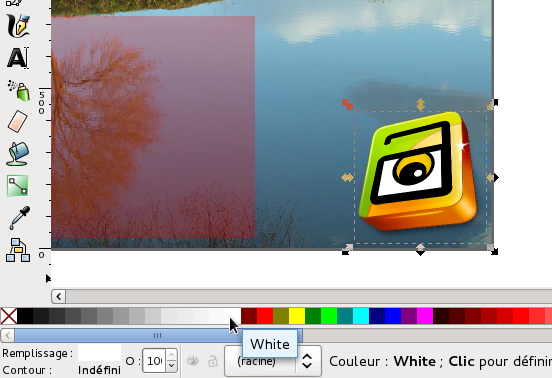
\includegraphics[width=0.6\textwidth]{images/remplissage_blanc}
 \label{remplissage_blanc}
\end{figure}

En indiquant une url dans le champs \chemin{Titre} des \chemin{Propriétés de l'objet}, l'image incorporée
devient une icône clicable renvoyant vers la page web en question.

\subsection{Afficher une question et accéder à une réponse}

Pour insérer dans un détail un bouton «~\textit{Réponse}~» clicable bloquant momentanément l'accès à la suite du commentaire,
rien de plus simple!

Il suffit en effet d'insérer dans la description, à l'endroit souhaité, la ligne\\
\verb|Réponse:| ou \verb|réponse:| et de rédiger en-dessous le texte que l'on souhaite voir apparaître.

\subsection{Contrôler le comportement des détails: affichage immédiat et désactivation
de l'effet «~zoom~»}\label{couche_XML}

Par défaut, le comportement d'un détail dans l'image active générée est le suivant:
\begin{itemize}
 \item Le détail ne se révêle qu'au survol de la souris ou qu'à la sélection du titre du commentaire
 qui lui est associé
 \item Un second clic sur un détail déjà sélectionné effectue un zoom sur celui-ci\footnote{À l'exception
 du modèle d'export popBlue.	}
\end{itemize}

Ces deux comportements sont modifiables par l'application, dans Inkscape, d'un fond de couleur blanche ou noire
aux détails détourés (voir section \ref{insertion_images} et figure \ref{remplissage_blanc}):
\begin{description}
 \item [Détail auquel est appliqué un fond de couleur blanche] Dans l'image générée, 
 le détail sera immédiatement visible, sous la forme d'un aplat de couleur opaque (masquant
 logiquement l'image de fond), qui une fois sélectionné, révêle l'image de fond (le détail demeure zoomable)
 \item [Détail auquel est appliqué un fond de couleur noire] Le détail n'est visible qu'en étant sélectionné, mais
 n'est pas zoomable.
\end{description}

Conséquence logique: un détail ne pouvant se voir appliquer à la fois un fond blanc et noir, il ne peut être à la
fois immédiatement visible \textit{et} non-zoomable.

\subsection{Contrôler l'ordre d'affichage des détails dans l'image active}

Par défaut, dans l'image active générée, les détails apparaissent verticalement dans l'ordre 
dans lequel les détails correspondants ont été créés (le premier détail créé dans Inkscape 
correspondant au détail placé en haut dans la barre latérale de l'image active).

On passera par l'\chemin{Éditeur XML} dans le menu \chemin{Édition} pour modifier cet 
ordre par défaut.

A priori complexe à gérer, cette fenêtre de dialogue se laisse en réalité apprivoiser aisément: 
la sélection sur l'image des détails met en évidence les entrées XML correspondantes, qu'il n'y 
a donc plus qu'à les glisser-déposer à l'endroit désiré (voir figure \ref{ordre_couches}).

De ce fait, l'utilisateur qui modifie fréquemment l'ordre de ses détails devrait prendre l'habitude 
de renseigner pour chacun d'eux le champs \chemin{ID} de ses propriétés, afin d'être en mesure 
de le manipuler plus aisément dans l'\chemin{Éditeur XML}.

\begin{figure}[htp]
 \centering
 \caption{L'éditeur XML d'Inkscape permettant de contrôler l'ordre d'affichage des détails dans l'image 
 active générée. On remarquera la mise en évidence d'un élément dans l'éditeur et sur l'image de fond 
 par simple clic de souris.}
 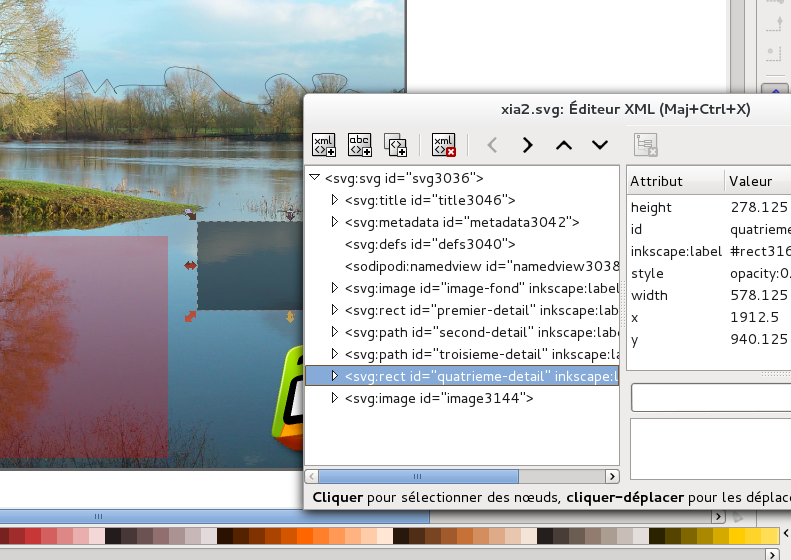
\includegraphics[width=\textwidth]{images/ordre_couches}
 \label{ordre_couches}
\end{figure}

\subsection{Pour résumer}

\begin{enumerate}
 \item On peut enrichir et mettre en forme le texte en utilisant des balises
 \item Un enrichissement multimédia est possible par un simple lien relatif ou absolu vers un fichier 
 dont le format est reconnu par Xia
 \item L'ajout d'images sur l'image de fond est possible par simple importation de celles-ci
 \item On modifie le comportement par défaut d'un détail en changeant sa couleur de fond (blanc, noir)
 \item L'ordre des détails dans l'image active générée dépend de l'ordre de création de ceux-ci, 
 mais reste modifiable via l'éditeur XML d'Inkscape
\end{enumerate}


\section{De l'interactivité à l'activité: réaliser des jeux avec Xia}

Jusqu'à présent, cette documentation a uniquement abordé la réalisation d'images actives au sens «~traditionnel~»:
une image de fond dont des détails détourés sont associés à des commentaires plus ou moins enrichis.

Ce type d'image permet de mettre en œuvre des scénarios pédagogiques ne manquant pas d'intérêt 
(découverte progressive de documents, fabrication par les élèves d'images actives), 
mais Xia va beaucoup plus loin en permettant la réalisation de jeux et d'activités variées, dans lesquelles
l'utilisateur est amené à réaliser infiniment plus d'actions que la simple lecture
 de commentaires...

\subsection{Premier principe ludique: sélectionner, retrouver dans l'image}

Explorez l'\href{http://geoffrey-gekiere.ac-versailles.fr/xia3}{image active créée pour cette section de la documentation} 
et téléchargez le \href{http://geoffrey-gekiere.ac-versailles.fr/xia3/svg/xia3.svg}{svg}.

\textit{Le principe ludique est le suivant: on propose une image dans laquelle l'utilisateur 
doit sélectionner un certain nombre de détails en fonction d'une consigne. 
La réalisation de l'objectif énoncé déclenche l'affichage d'un message.}

C'est en réalité l'activité, voire l'image active la plus simple à réaliser. Il suffit en effet 
au créateur de la ressource de détourer les éléments que l'utilisateur doit retrouver.

La consigne à destination de l'utilisateur de l'image active est à renseigner 
dans les métadonnées du document. En effet, au moment de l'export, Xia cherche les informations
situées dans le champs \chemin{Description} des métadonnées du document 
(voir section \ref{preparation_svg} et figure \ref{titre_ia}), afin d'en faire une «~pop up~»
qui s'affichera lors de l'ouverture de l'image générée. L'utilisateur lit alors la consigne et ferme
la pop up pour jouer.

Lorsque l'utilisateur a réussi le jeu, un message apparaît. 
Celui-ci est créé dans la \chemin{Description} des \chemin{Propriétés de l'objet} de l'image de fond
\footnote{Quand une image active «~traditionnelle~» est générée, cette manipulation
permet la création du commentaire introductif à l'image, non relié à un détail particulier
(voir section \ref{preparation_svg}).}. 
Deux informations sont nécessaires pour que ce message apparaisse:
le nombre de bonnes réponses déclenchant le message\footnote{Ce nombre est à la discrétion
du créateur de la ressource et peut tout à fait être inférieur au nombre total de détails placés sur l'image},
et le message en lui-même. Ce tableau résume les balises à insérer:

% le multicolumn refuse le \verb... à corriger
\begin{center}
 \begin{tabular}{|l|p{2in}|p{2in}|}
 % \hline
% \multicolumn{3}{|c|}{Informations à renseigner dans le champs Description des Propriétés de l'objet}\\
 \hline
  Objectif & Renseigner le nombre de bonnes réponses nécessaires pour terminer le jeu & Afficher un message\\
  \hline
  Balise & \verb|<score></score>| & \verb|<message></message>|\\
  \hline
  Exemple & \multicolumn{2}{|l|}{<score>6</score>}\\
   & \multicolumn{2}{|l|}{<message>Bravo, vous avez réussi à sélectionner}\\
    & \multicolumn{2}{|l|}{correctement tous les éléments demandés</message>}\\
  \hline
 \end{tabular}
\end{center}

Astuce: le texte inséré dans la balise \verb|<message></message>| peut 
tout à fait être enrichi. 
On peut ainsi imaginer de proposer le visionnage d'une image, d'une vidéo, ou l'affichage d'un lien vers un second exercice, afin 
de «~chaîner~» les activités par degré de difficultés.

La génération d'une l'image active ayant pour principe ludique la sélection de détails
correspond dans Xia à l'export \chemin{game1clic}:

\begin{center}

\includegraphics[scale=0.7]{./images/game1clic} 
\end{center}

\subsubsection{Pour aller plus loin... Comment montrer à l'utilisateur sa progression lors de l'utilisation d'un jeu game1clic?}\label{detail_progression}

On peut programmer l'apparition d'éléments visuels lorsque l'utilisateur sélectionne une réponse correcte. 
Ces éléments peuvent être issus de l'importation d'images au format png, mais également 
être directement créées dans Inkscape.
Cependant, puisque Xia considère comme un détail clicable tout élément créé à partir des outils 
d'Inkscape, il faudra, après avoir dessiné ceux-ci, les transformer en «~copie bitmap~».
Par exemple:
\begin{enumerate}
 \item On dessine une étoile de côtés jaune sur fond jaune avec les outils d'Inkscape
 \item Après avoir sélectionné cette étoile, on clique, dans le menu \chemin{Édition}, sur 
 \chemin{Faire une copie bitmap}
 \item On supprime l'étoile ayant servi à créer cette copie bitmap, devenue inutile
\end{enumerate}

Une fois les éléments visuels importés (fichiers png) ou créés (copie bitmap de figures créées à la main),
il suffit d'appliquer à ceux-ci la caractéristique
\begin{center}
\chemin{Interactivité > OnClick} = \verb|off|
\end{center}
et enfin de grouper le détail clicable à cet élément (en cliquant successivement sur le détail et l'élément visuel en maintenant 
la touche Maj enfoncée, puis en sélectionnant \chemin{Grouper} dans le menu \chemin{Objet} d'Inkscape).

\subsubsection{Pour aller plus loin... Comment mettre en évidence les erreurs de l'utilisateur dans un jeu game1clic?}

Le principe ludique de la sélection d'un ensemble de détails dans une image a un intérêt pédagogique évident... 
et des limites qui le sont tout autant (on imagine aisément un élève tenter de cliquer frénétiquement sur chaque pixel 
de l'image active sans réfléchir une seule seconde...).

C'est la raison pour laquelle il peut être intéressant d'être en mesure de mettre en évidence dans le jeu les erreurs commises 
par les utilisateurs.

Pour cela, le créateur de la ressource prévoiera de déposer aux endroits stratégiques de son image de fond, dans Inkscape, 
un élément visuel assez explicite pour symboliser l'erreur. Cet élément visuel peut être une 
image au format png ou une forme créée directement avec les outils de dessins d'Inkscape, puis transformée en bitmap 
(voir la méthode décrite à la section \ref{detail_progression}). 
On appliquera à celui-ci la caractéristique
\begin{center}
\chemin{Interactivité > OnClick} = \verb|disable-score| 
\end{center}
De cette manière, le détail demeure
clicable, mais son activation n'ajoute pas un point au compteur permettant au final de déclencher 
le message de victoire.

\subsection{Second principe ludique: classer, légender, hiérarchiser}

\textit{Second principe ludique: une image de fond contient des étiquettes qu'il faut déplacer et 
déposer sur les bons détails. Lorsque tous les éléments ont été remis à leur place, un message 
confirme la résolution du jeu.}

Explorez l'\href{http://geoffrey-gekiere.ac-versailles.fr/xia5}{image active créée pour cette section de la documentation} \\
et téléchargez le \href{http://geoffrey-gekiere.ac-versailles.fr/xia5/svg/xia5.svg}{svg}.

La démarche pour la réalisation d'un jeu de ce type est la suivante:
\begin{enumerate}
 \item Dans Inkscape:
\begin{itemize}
 \item Choisir une image de fond
 \item Préparer les «~étiquettes~» à déplacer (petites images ou texte)
 \item Faire correspondre chaque étiquette à sa zone de dépôt (en réalité, un détail détouré)
 grâce aux métadonnées renseignées
\end{itemize}
 \item Dans Xia
 \begin{itemize}
  \item Exporter le svg ainsi préparé avec le thème «~gameDragAndDrop~»
 \end{itemize}
\end{enumerate}

Deux méthodes sont envisageables pour disposer des «~étiquettes~» à déplacer.
Un moyen simple est d'utiliser un utilitaire de capture d'écran 
capable de produire des images au format png puis d'importer celles-ci dans Inkscape.
On peut également produire des étiquettes de type texte directement dans Inkscape en regroupant un 
cadre (outil \chemin{Créer des rectangles et des carrés}) et un élément textuel puis en 
faisant une copie bitmap de cet ensemble (voir section \ref{detail_progression})\footnote{... sans oublier, après avoir
fait la copie bitmap, de supprimer le regroupement devenu inutile.}.
On fait ensuite correspondre aux détails censés les accueillir\footnote{\textbf{Une} étiquette ne pouvant correspondre qu'à \textbf{un} détail.}.

Le tableau suivant résume les métadonnées à renseigner dans les \chemin{Propriétés de l'objet}
dans l'étiquette et le détail correspondant afin de les «~jumeler~»:

\begin{center}
\begin{tabular}{|p{1.in}|p{2.5in}|p{1.5in}|}
\hline
 & Étiquette (objet à déplacer) & Détail détouré (réceptacle de l'étiquette)\\
\hline
Champs ID & & \verb|Titre_Detail|\\
\hline
Champs Description & \verb|<target>Titre_Detail</target>| & \\
\hline
Champs Interactivité > Onclick & & \verb|off|\\
\hline
\end{tabular}
\end{center}

Pour résumer, le créateur de la ressource fait savoir à Xia quelle étiquette correspond à quel détail en faisant 
correspondre le champs \chemin{ID} du détail (réceptacle) au champs \chemin{Description} de l'étiquette 
(objet à déplacer). La seule subtilité consiste à entourer, dans le champs \chemin{Description}
de l'étiquette, l'ID correspondante d'une balise \verb|<target></target>|.

Une astuce: si l'image active contient de nombreux détails réceptacles de taille identique, 
on peut en créer une, lui appliquer la caractéristique \chemin{Interactivité > OnClick} = \verb|off|, 
puis copier-coller ce détail autant de fois que nécessaire. Conservant cette option, 
le créateur de la ressource n'aura pas besoin d'aller l'appliquer à chaque détail créé, 
et aura uniquement à modifier les champs \chemin{ID}.

La génération d'une l'image active ayant pour principe ludique le glisser déposer 
correspond dans Xia à l'export \chemin{gameDragAndDrop}:

\begin{center}

\includegraphics[scale=0.7]{./images/gameDragAndDrop} 
\end{center}

\subsubsection{Comment ajouter un effet «~magnétisme~» dans le jeu gameDragAndDrop}

En indiquant\\
\begin{center}
\verb|<magnet>on</magnet>| 
\end{center}
dans le champs \chemin{Description}
du détail réceptacle de l'étiquette, un effet «~aimant~» sera effectif au moment où 
l'utilisateur approche son étiquette de la cible.

L'avantage de cette option est qu'elle permet à l'utilisateur d'être sûr que 
la non-résolution du jeu provient d'une erreur de correspondance de ses 
étiquettes, et pas d'un léger décalage entre l'étiquette et la zone de dépôt.

\subsection{Pour résumer}

Aperçu synthétique des principales balises à insérer dans le cadre de
la création d'un jeu (export game1clic ou gameDragAndDrop):

\begin{center}
 \begin{tabular}{|p{1.5in}|p{1in}|p{1in}|p{1in}|p{1in}|}
 Balise & Quel rôle? & Sur quel objet? & À insérer dans... & Qu'y insérer?\\
 \hline
 \verb|<score></score>| & Indiquer le nombre de bonnes réponses déclenchant le message de fin & Image de fond & Propriétés de l'objet > Description & Le chiffre correspondant au score demandé\\
 \hline
 \verb|<message></message>| & Afficher le message de fin du jeu & Image de fond & Propriétés de l'objet > Description & Un message personnalisé, si besoin enrichi\\
 \hline
 \verb|off| & Rendre insensible au clic un détail & Détail & Propriétés de l'objet > Interactivité > Onclick & \\
 \hline
 \verb|disable-score| & Conserve la sensibilité au clic mais n'ajoute pas de point au compteur de résultat quand sélectionné & Détail & Propriétés de l'objet > Interactivité > Onclick & \\
 \hline
 \verb|<target></target>| & Indique au détail déplaçable son détail fixe correspondant & Détail à déplacer & Propriétés de l'objet > Description & Faire correspondre au champs ID de la cible\\
 \hline
 \verb|<magnet>on</magnet>| & Ajoute un effet «~aimant~» & Détail réceptacle & Propriétés de l'objet > Description & \\
 \end{tabular}
\end{center}


\end{document}